%Het eerste hoofdstuk van je thesis.
\chapter{Literatuurstudie}
De literatuurstudie schetst een beeld van de sateliet constellaties die gebruikt worden. Deze worden besproken in \ref{LGNS}. Eens we de verschillende types van satelieten kennen, besrpeken we de manier waarop ze met elkaar communiceren in sectie \ref{LCom}.

\section{GNSS}
\label{LGNS}
GNSS ofwel Global Navigation Satellite System, is een sateliet systeem met een wereldwijde dekking. GNSS is een standaard term gebruikt om systemen te beschrijven die positie en navigatie oplossingen bieden. HEt werd voornamelijk ontwikkeld voor de luchtvaart en ruimtevaart industrie en militaire doeleinden. Tegenwoordig worden deze technologieën ook in andere toepassingen gebruikt. GNSS vraagt samenwerking tussen verschillende publieke en private organisaties \cite{LBibGNSS3}.  Dit systeem is opgebouwd uit verschillende subsystemen die verder in deze tekst bepsroken worden. Namelijk: GPS besproken in sectie \ref{LGPS}, In sectie \ref{LGLO} bespreken we GLONASS, Galileo wordt besproken in sectie \ref{LGal} en BeidDou komt al laatste aan bod in sectie \ref{LBeD}. Het IGS, International GNSS Service staat in voor de aflevering van de hoogste kwaltieit GNSS data en producten \cite{LBibGNSS}. Elke satelliet is een project op zichzelf. Hierdoor is het moeilijk om een gestandaardiseerde productie ketting te creëren \cite{LBibGNSS3}.

\subsection{GPS}
\label{LGPS} 
GPS staat voor Global Positioning System. Dit is het satelieten gebaseerde positie systeem dat bij ons het bekendste is. Het is ontwikkeld in Amerika \cite{LBibGNSS}\cite{LBibGNSS3}. Voor de gebruikers is kost van de data een hoge bezorgdheid. Daarom is het belangrijk om de kosten van de operaties te verkleinen. GPS moet toegankelijk zijn voor meerdere clients. De gebruikerstoegang gebeurt voornamelijk door mobiele toestellen die verbingig maken via het internet \cite{LBibGPS}.

\subsubsection{Manieren om posities te bepalen}
\paragraph{Differential GPS Corrections}
Differential GPS Corrections ook weel DGPS genoemd, worden gebruikt om nauwkeurig posities  te bepalen. Er worden minimaal twee GPS ontvangers gebruikt. Van \'e\'en van deze ontvangers moet de preciese postie gekend zijn. De positie van het andere station kan dan geschat worden door een vergelijking van de co\"ordinaten van de twee stations. Dit is een populaire manier om sateliet en klok fouten te elimineren. Een nadeel van deze techniek is dat de observaties van beide stations simultaan moeten gebeuren \cite{LBibGNSS2}. 


\subsection{GLONASS}
\label{LGLO}

\subsection{Galileo}
\label{LGal}
Galileo is het Europees systeem \cite{LBibGNSS3}.

\subsection{BeiDou}
\label{LBeD}

\section{Communicatie}
\label{LCom}
\subsection{Euref Permanent Netwerk}

\subsection{RTCM}

\subsection{NTRIP}
\label{LNTR}
Networked Transport of RTCM via Internet Protocol of kortweg NTRIP. Men maakt gebruik vant internet om de realtime GNSS data uit te wisselen en te verzamelen. NTRIP is een HTTP(Hypertext Transfer Protocol) stateless applicatie level protocol om GNSS data te streamen over het internet. De nodige brandbreedte hiervoor is niet groot in vergelijking met bijvoorbeeld Internet Radio\cite{LBibNTRIP}. Het is gebaseert op software die oorspronkelijk bedoelt was voor MP3 media speler formaten. Dit blijk wel aangepast te zijn voor GNSS stromen met data snelheden toosen 0.5 en 5 kbit/s. \cite{LBibGPS}. Een ander voordeel is dat tegenwoordig op veel plaatsen internet verbinding voorzien is \cite{LBibNTRIP}

\subsubsection{opbouw van NTRIP software}
\label{LONS}
NTRIP wordt ge\"implemeneteerd in drie systeem software componenten. Nameijk Ntrip clients, NtripServers en NtripCasters. De NtripCaster is het HTTP server programma terwijl NTRIPClients en NTRIPServers reageren zoals HTTP clients\cite{LBibNTRIP}. NTRIPServers gaat datastromen vervoeren. NTRIPCasters gaan de administratie tussen clients en datastromen afhandelen \cite{LBibGPS}. NTRIPCasters is een stream-spliteser en broadcaster component, momenteel zijn er acht NTRIPCasters in Europa. NTripClients gaan data ontvangen van de gewenste bronnen via de NTRIPCaster. NTRIPServers gaan de data van \'e\'en of meerdere bronnen verzenden in NTRIP formaat. Als laatste hebben we ook nog NTRPSorurces, deze genereren DPGS datastreams op een specifieke locatie. \cite{LBibNTRIP} In figuur \ref{imgNTRIP} staat een overzicht van de opbouw van het NTRIP streaming systeem.

\begin{figure}[hpb]
	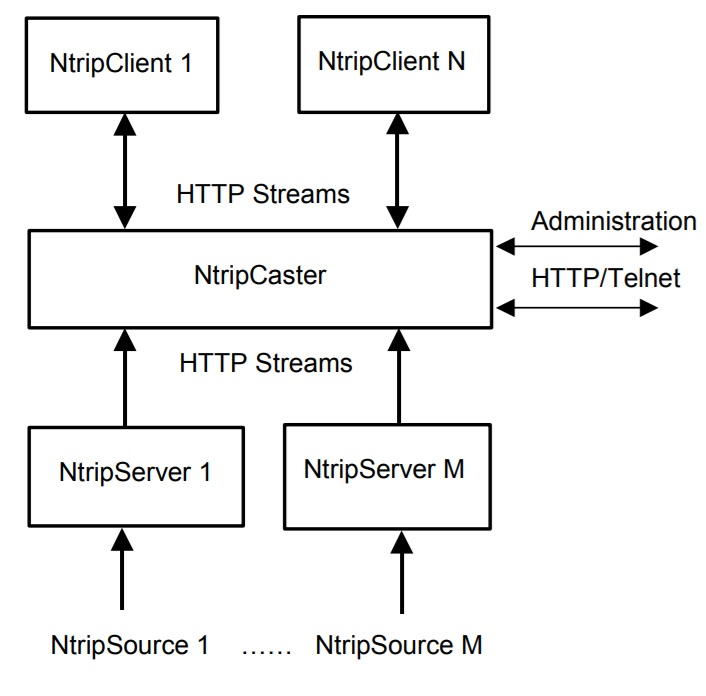
\includegraphics[scale=0.75]{NTRIP.jpg}
	\caption{NTRIP streaming systeem}
	\cite{LBibNTRIP}
	\label{imgNTRIP}
\end{figure} 
 



